\documentclass[a4paper,12pt,titlepage]{article}

\usepackage{listings}
\usepackage{amsmath}
\usepackage{amssymb}
\usepackage{amsthm}
\usepackage{graphicx}
\usepackage{hyperref}
\usepackage{parskip}

\setlength{\parindent}{15pt}

\begin{document}

\title{Network Security Class \\ Lab Session 1}
\author{Stefano Zanella - 621796}
\date{July 2013}

\maketitle

\section{Assignment}
A C and Matlab codebase is given, containing the implementation of a linear and
a nearly-linear Feistel ciphers, plus three sets of plaintext/ciphertext pairs for
different cipher instances and keys. The assignment is as follows:
\begin{itemize}
  \item implement the \texttt{feistel\_decrypt} procedure;
  \item carry out a KPA on the linear Feistel cipher with 8 rounds and 32 bit
        key and plaintext;
  \item carry out a KPA on the nearly linear Feistel cipher with 4 rounds and 8
        bit key and plaintext, and evaluate its success rate;
  \item carry out a KPA on the nearly linear Feistel cipher with 2 rounds and
        32 bit key and plaintext, and evaluate its success rate.
\end{itemize}

\newpage

\section{Implementing the decryption procedure}
Instead of copy/pasting the code, I slightly modified the original
\texttt{feistel\_encrypt} function so that it can work 
\emph{both as an encryptor and as a decryptor} (thus renaming it 
\texttt{feistel\_encdec}). \\
Since the only difference in encryption and decryption algorithms is the order
in which subkeys are generated (one being the reverse of the other), it
seemed almost natural to try to implement a single procedure with the
capability of accepting a flag that can reverse the order of the subkey
generation.

To do this, we need to manipulate the \texttt{subkey\_cyclic\_rotation} function, since
its original implementation is \emph{"round-agnostic"}: that is, its output depends
only on the current input but not on the round number. This is a correct
formulation that strictly resembles the general block diagram of a Feistel
cipher, but it doesn't allow us to get keys in reversed order if not by
generating all the keys upfront and iterating over them backwards. Looking at this
function with a more software-oriented eye, though, we can see that it can be
modified so that its output can be \emph{"round-aware"}. \\
In fact, the output of this function is built by splitting the
input array into two halves and by rotating them "outward" by 1 bit (1 bit
\texttt{ROL} for 1st half, 1 bit \texttt{ROR} for 2nd half). \\
If we compare the output of this function at round $j$ with the
original key $k$,
we see that the subkey $k_j$ is just the original key $k$, splitted in two halves
and outward-rotated by $j$ bits (assuming $j$ starts from 1).
This tells us that if we parametrize the amount of bits rotated by the 
function, we can obtain a general subkey $k_j$ with a single call. \\
The resulting function is called \texttt{half\_outward\_shift}; to use it in the
new Feistel encryptor/decryptor procedure, we need to modify the code so that
it passes the correct parameters to it.

If we just want to retain the original behavior of the \texttt{feistel\_encrypt} 
function, we only need to eval at each round \texttt{subkey\_generation} with the
original key and round number as parameters. \\
However, we also need to use the same cycle to perform ciphertext decryption. \\
This can be done by replacing the plain round number $i$ passed to the subkey
generation function with the function $abs(i - D)$, where
$D$ is a constant that
evaluates to \texttt{0} if we want to encrypt the input, and to \texttt{nr\_rounds} if we're
going to decrypt the message.

As a recap, we:

\begin{itemize}
	\item created a new subkey generation function \texttt{half\_outward\_shift} which can
        calculate subkey $k_j$ with a single call starting from original key and round
        number
	\item renamed \texttt{feistel\_encrypt} to \texttt{feistel\_encdec} and modified it so that it can
        perform both encryption and decryption by setting a flag parameter
	\item wrapped calls to \texttt{feistel\_encdec} into two helper functions \texttt{feistel\_encrypt}
	      and \texttt{feistel\_decrypt}
\end{itemize}

To prove that the resulting code is correct, it is sufficient to perform the
decryption of the encrypted message a certain number of times over a certain
number of random messages and see that the result of the composition of the
functions equates to the original message:

\begin{lstlisting}[language=Matlab]
for i = 1:very_large_number
  msg = dec2hex(randi([0,2^32-1],1,1))
  assert(isequal(
    msg,
    feistel_decrypt(
      feistel_encrypt(msg, key, 4, ...
        @linear_round_function, @half_outward_shift), 
      key, 4, @linear_round_function, @half_outward_shift),
    'u and u_hat are supposed to be equal'))
end
\end{lstlisting}

\section{Linear cryptanalysis}
\subsection*{Mathematical model}
Since it's a given assumption that the cipher implemented using
\texttt{@linear\_round\_function} is indeed linear, we can treat the encryptor as a
linear system and analyze it with the binary version of a \emph{pulse train}. In our
case, given 
$k \in \mathbb{B}^{32},\: u \in \mathbb{B}^{32},\: x \in \mathbb{B}^{32}$
(respectively, the key, plaintext message and
ciphertext), we can model the encryptor as:
\[x = \mathbf{A}k + \mathbf{B}u \] 
where $\mathbf{A}$ and $\mathbf{B}$ are two $(32 \times 32)$
square matrices such that $\mathbf{A},\mathbf{B} \in \mathbb{B}^{32} \times \mathbb{B}^{32}$.

That said, under the assumption that $\mathbf{A}$ is non-singular we
can find the solution of the linear system for a given known
plaintext-ciphertext as:
\[k = \mathbf{A}^{-1}(x - \mathbf{B}u)\]

In this case, since the system is linear, we need to solve this system only for
one given plaintext-ciphertext pair. Solving the system for all the other pairs
must give the same key.

\subsection*{System Analysis}
With this structure in mind, we now have to derive the two matrices from the
practical implementation to fill in the model and actually obtain the
information we're looking for. \\
Deriving the two matrices can be done in two symmetric steps that apply the
following idea to both the plaintext and the key:

\begin{enumerate}
	\item We set one of the two inputs of the encryptor block to the 4-words binary
        representation of \texttt{0} (i.e. \textbf{\texttt{00000000}})
	\item We let the other input to be the binary representation of the number \texttt{1},
        also as a 4-word message (i.e. \textbf{\texttt{00000001}})
	\item We run the encryptor with these particular inputs. It can be easily seen
        that the output is the value of the 31st column of either the
        $\mathbf{A}$ or $\mathbf{B}$ matrix, depending on how we
        initialized the inputs
	\item We iterate all of the above over the inputs updated as follows:
    \begin{itemize}
      \item The input set to \texttt{0} remains the same
      \item  The pulse input is left-shifted by 1 bit.
    \end{itemize}
\end{enumerate}

If we memorize the columns obtained as ciphertexts, after shifting the pulse
array by its whole length we can obtain the full $\mathbf{A}$ or
$\mathbf{B}$ matrix. Then, we can just perform the same procedure
another time swapping the roles of the two inputs to obtain the other missing
matrix.

\subsection*{Implementation Caveats}
We developed our model under the assumption of matrix $\mathbf{A}$
being invertible. Unfortunately, it turns out that with the given Feistel cipher
implementation, the key multiplication matrix doesn't have full rank but
instead has \textbf{2 linearly dependent} rows/columns. This prevents us to invert
the $\mathbf{A}$ matrix. Still, we can get over this problem by using Gaussian
elimination over a Galois field, provided by the \texttt{gflineq} function (see
References).
It is worth noting how this little complication in the resolution of the
system eventually proves the cipher to be even weaker than supposed: in fact,
since $rank(\mathbf{A}) = 30$, for each given key, there are $2^2-1$ that
represent the same exact map between message and ciphertext spaces. This mean
one could reduce the search space by a factor 4 in case of a bruteforce attack.
This doesn't give a direct advantage to the cryptanalyst
in this case, since solving the linear equation is a more efficient way to
break the system than bruteforcing; however, it will be shown later how this helps in breaking
the nearly-linear Feistel cipher.

\subsection*{Equivalent Keys}
Given the last observation it's also worth noting how we can find the set of
equivalent keys corresponding to a particular solution. \\
The focal point is the XORing of the key bits in the round function. Basically,
we can see from the truth table of the XOR function that given two bits $x$
and $y$, $x \oplus y = \bar{x} \oplus \bar{y}$. This in itself means that given
any input, encrypting or decrypting with a key produces the same output of
applying the same operation with its \textbf{bitwise complement}. \\
Furthermore, if we look at the cipher implementation, we notice that the subkey generation
function treats the key as two independent halves (bits belonging to one half
of the key never end up in the other half after subkey generation). At the same
time, the round function relates each bit of the input with two
\textbf{adjacent} bits of the key. Putting these two last observations
together, we obtain that the composition of the round function and subkey
generation is done independently on the two halves of the key and the input.
This, combined with what already said, means that we can obtain equivalent keys
by picking for each half of the key \textbf{its original form or its bitwise
complement}. It's easy to see how this freedom partitions the key space in sets of
equivalent keys each of size 4.

To better explain, let's look at an example. Given a key
\begin{verbatim}
12345678 == 0001001000110100|0101011001111000
\end{verbatim}
its equivalent are:
\begin{verbatim}
EDCBA987 == 1110110111001011|1010100110000111
1234A987 == 0001001000110100|1010100110000111
EDCB5678 == 1110110111001011|0101011001111000
\end{verbatim}

\subsection*{Attack Implementation}
The impulse response of the system is calculated in the \texttt{impulse\_response}
function. It outputs the two matrices $\mathbf{A}$ and
$\mathbf{B}$. This function is then called by the
\texttt{feistel\_linear\_cryptanalysis} script, which calculates the key for the first
known-text pair and then compares it with the other known pairs as a proof of
correctness.

The key resulting from running the cryptanalysis script with the KPA set \#3 is:
\begin{verbatim}
  C3F8177E
\end{verbatim}

and its equivalent are:
\begin{verbatim}
  3C07E881
  3C07177E
  C3F8E881
\end{verbatim}

\section{Nearly-linear cryptanalysis (4 rounds, 8 bits)}
\section{Nearly-linear cryptanalysis (2 rounds, 32 bits)}
Since only 2 rounds are performed here, we can use a \emph{meet in the middle}
technique. \\
That is, we can exploit the relation between plaintext and ciphertext and try
to invert this relation in a fashion similar to what we've done with the linear
cipher.

Let's start by analyzing the structure of the particular Feistel cipher under
the circumstances given by the assignment. \\

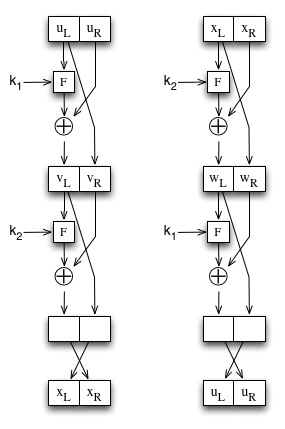
\includegraphics{2_rounds_feistel.jpg}

By looking at the figure, we can setup the following equations (2 pairs for the
encryptor, 2 pairs for the decryptor):
\[v_L = F(u_L, k_1) \oplus u_R \qquad v_R = u_L \qquad x_R = F(v_L, k_2) \oplus v_R \qquad x_L = v_L\]
\[w_L = F(x_L, k_2) \oplus x_R \qquad w_R = x_L \qquad u_R = F(w_L, k_1) \oplus w_R \qquad u_L = w_L\]

Then, by expanding the first 4 equations we see that:
\[ x_R = F(v_L, k_2) \oplus u_L \qquad x_L = F(u_L, k_1) \oplus u_R \]
\[ x_R = F(x_L, k_2) \oplus u_L \qquad x_L = F(u_L, k_1) \oplus u_R \]

Then, by XORing on both sides of the equations we obtain:
\[x_L \oplus u_R = F(u_L, k_1)\]
\[x_R \oplus u_L = F(x_L, k_2)\]

The same result can be obtained by exploting the relationships in the last 2
pairs of equations coming from the decryptor's model.

We can see how the left term of both equations is well-known; if we had a way
to calculate the inverse of the round function with respect to the two subkeys,
then we could simply retrieve the key given one known text pair. This, however,
can't be done in this case in a deterministic way since the round function is
non-linear. Nonetheless, we can make the relation between the round function's
arguments explicit and see that we can still gather few bits of information
given a known text pair. We begin by writing down the bitwise expression for F.
Given:
\[w = F(k, y)\]
and
\[w = w_{15} \; w_{14} \; ... \; w_1 \; w_0\]
\[y = y_{15} \; y_{14} \; ... \; y_1 \; y_0\]
\[k = k_{31} \; k_{30} \; ... \; k_1 \; k_0\]
then
\[w_{2j} = y_{2j} \vee (k_{2j} \oplus k_{2j+1})\]
(that is, each output bit is the OR between the input bit at same position and
the XOR of a pair of adjacent bits of the key).

That said, we can look at the truth table of the OR function and infer the
following:
\[\forall j : y_{2j} = 0 \Rightarrow k_{2j} \oplus k_{2j+1} = w_{2j}\]
so, we have a way to infer valid linear equations between bits of the key (note
that we have to account for different subkeys being used in different rounds;
this is easy to handle since we know how the bits positions change between
subkeys). \\
We can then collect each valid equation and put it in a system; in the ideal (from
the attacker standpoint) case, we then obtain a full rank system of linear
equations that can be easily solved to recover all key bits. \\
However, since there's no guarantee of obtaining a good amount of linearly
independent equations, we need to account for a certain amount of freedom when
solving the system.

In fact, in the given case, applying this technique holds a matrix of rank
\textbf{29} instead of the expected \textbf{30}. In should be noted that,
whatever the rank obtained, any particular solution of the given system will
correctly encrypt all known plaintexts into their corresponding known
ciphertexts (and viceversa); this result holds by construction of the linear
equation system itself. However, unless the rank is full, we still can't be sure
that a particular key solving the system is the \emph{right} key we're looking
for. \\

A step further can be done in this direction by trying to list \emph{all} keys
satisfying the system. This can be done by
collecting those expressions that didn't allow us to infer valid equations for
the system during the discovery phase; then, they can be appended to the matrix by
manually setting the corresponding constant each time at either $0$ or $1$.
This way we can perform a brute force attack just on the part of the problem we
can't gather information about. This allows to reduce the search space from
$2^{32}$ to $2$ keys.

This process has been implemented in two functions:
\texttt{find\_valid\_lineq\_for\_mitm} and \texttt{feistel\_mitm\_cryptanalysis}. The
first discovers all equations for a given plain-ciphertext pair, returning two
matrices, one containing valid equations and one containing the expressions
representing the degree of freedom. \\
The second function, instead, iterates over all given text pairs building the
overall system of linear equations, then applying those that have free
constants and solving it iteratively, each time setting the free constants to a
different value.

In the particular case solved with this technique,
\texttt{find\_valid\_lineq\_for\_mitm} were able to find $75$ equations over the
key bits, put into a matrix of rank $29$, and $2$ equations with unkown
constant value. For $2$ instances of the $4$ possible systems obtainable by
setting the unknown constants, there were no solution; the other two, instead,
provided the two expected keys; these keys, in turn, given the considerations
done in the preceding sections, form a set containing them, their complements
and combinations of the two. As a result, we can say that the key used to produce the
given text pairs belong to the following set:
\begin{verbatim}
E176A1CE
1E895E31
E1765E31
1E89A1CE
1E76A1CE
E1895E31
1E765E31
E189A1CE
\end{verbatim}

Furthermore, given the considerations about equivalent keys, we can state that
the set is composed of $2$ partitions, each containing $4$ equivalent keys, so
with just the given set of known text pairs if we pick a key to decrypt further
transmissions the success rate is $50\%$ (or $100\%$ if we consider decrypting
with two distinct keys and under the assumption we can discriminate between
good and bad decrypted messages).

\section{References}
\begin{itemize}
  \item Since in Octave there isn't a function to solve systems of linear equations
        over a Galois Field, a function \texttt{gflineq} has been added, whose original
        implementation has been found at: \\
        \url{http://read.pudn.com/downloads64/sourcecode/others/224341/ldpc_toolkit/gflineq.m__.htm}.
\end{itemize}
\end{document}
